\documentclass[11pt,dvipsnames]{article}

\usepackage{geometry}
\geometry{total={170mm,240mm}, left=20mm, top=20mm}

\usepackage[utf8]{inputenc}

\usepackage{physics} 
\usepackage{siunitx} 
\usepackage{enumerate} 
\usepackage{pgfplots}
\usepackage{graphicx}
\usepackage{pgfplotstable}
\usepackage{tikz,pgfplots}
\usepackage{amsmath} 
\usepackage{xcolor}
\usepackage{float}
\usepackage{amsfonts}

\usepackage[]{lineno}  \linenumbers
\setlength\linenumbersep{3pt}
	

\usepackage{fancybox}
\usepackage{colortbl}
\usepackage{amsbsy}
\usepackage[draft,inline,nomargin]{fixme} \fxsetup{theme=color}
\FXRegisterAuthor{cp}{acp}{\color{blue}CP}
\FXRegisterAuthor{ja}{aja}{\color{RedViolet}JA}

\begin{document}

\title{Projective maps on a system of $n$ qubits} 
%Title should be concise and to the point  
\author{J. A. de León\\
				\small{supervised by C. Pineda}}


\date{\today}  

\maketitle


According to \cite{nielsen_chuang_2011}, an arbitrary density matrix on $n$  
qubits can be expanded as
\begin{align}
	\rho = \frac{1}{2^n}\sum _{\vec{v}} \Tr 
                  \qty( \sigma _{v_1} \otimes \sigma_{v_2} \otimes 
               \cdots \otimes \sigma_{v_n} \rho) \sigma _{v_1} \otimes 
             \sigma_{v_2} \otimes \ldots \otimes \sigma_{v_n},
	\label{rho}
\end{align}
where the sum is over vectors $\vec{v}=\qty(v_1,\cdots, v_n)$ with entries
$v_i$ chosen from the set $\{0,1,2,3\}$. We label the coefficients $\Tr \qty(
\sigma _{v_1} \otimes \sigma_{v_2} \otimes \cdots \otimes \sigma_{v_n}
\rho )$ as $r_{v_1, v_2,\ldots, v_n}$ to shorten the notation. 

The kind of maps that act on density matrices of the form \eqref{rho} that
we're interested in are those which leave invariant or erase  
components
in $\rho$ (i.e. $r'_{v_1, v_2,\ldots, v_n}=r_{v_1, v_2,\ldots, v_n}$ or
$r'_{v_1, v_2,\ldots, v_n}=0$, where the primed $r$'s refer to the 
components in the transformed density matrix $\rho '$). 

So far, with a numerical method we've characterized all 1 and 2 qubit maps, 
whereas for 3 qubits system we have studied some maps that leave invariant 1, 2,
3 and 4 coefficients in $\rho$. \newline

Our results exhibit the following features:
\begin{itemize}
\item Only a power-of-2 number of components may be left invariant by valid
			quantum channels. Nonetheless,
			not only the number of 
			coefficients to leave invariant is taken into account but actually
			which coefficientes are left invariant too.

\item 
The number of valid quantum channels according to the number of components
left invariant are shown in Figure \ref{fig:CCs-by-components}.

\begin{figure}[H]
	\centering
		\begin{tabular}{>{$n=}l<{$\hfill}*{12}{c}}
			1 &&&&&1&3&1&&&&&5\\
			2 &&&&1&15&35&15&1&&&&67\\
			3 &&&1&\colorbox{RedOrange}{63}&\colorbox{Yellow}{561}&?&\colorbox{Yellow}{¿561?}&
				\colorbox{RedOrange}{¿63?}&1&&&?
			\end{tabular}
			\caption{First column shows the number of qubits in the system. 
							Second column displays, from left to right, the number of valid 
							quantum channels that correspond to 
							$2^0, 2^1, \ldots, 2^{2n}$ components that are 
							left invariant in $\rho$. Finally, third column specifies the 
							total number of quantum channels.}
			\label{fig:CCs-by-components}
\end{figure} 

For 3 qubits the maps that leave invariant 16 components in $\rho$
have not been numerically analized, but we pressume there's a 
1-on-1 correspondence for the number of valid channels between those that leave
invariant 2 and 32 components, and similarly between those that leave 4 and 16
componentes invariant. This observation follows 
from the correspondence in the results for 1 and 2 qubits 
between quantum channels that leave invariant $2^k$ and $2^{2n-k}$, for 
$k=1, 2, \ldots, n$.
		
% \item The results are recursive by increasing the number of qubits in the
% system, i.e. the valid quantum channels for 2 qubits have to obey the valid
% quantum channels for 1 qubit. In more detail, 
%\item Valid maps for $n$ qubits must be valid for subsets of qubits. For example,
%the 2-qubits quantum-channels
%that leave invariant any of the coefficients of the form $r_{v_1,0}$ or
%$r_{0,v_2}$ have to obey the valid quantum channels found for 1 qubit. 
%This induces nice rules that are not accessible (we think) by considering 
%a single $2^n$-level quantum system. {\color{blue} [Nota]
%No entiendo la utilidad de este punto. Salvo la regla que nos permite ver si el canal es un producto tensorial de canales (o no), no se a que otras reglas se refieren. Claramente un producto tensorial de canales es tal que los 1s internos coinciden con los 1s en las orillas. Si se especificará mas este punto, propongo borrarlo, creo que mete ruido.}

%\janote{A mí no me convence la redacción del item anterior. A diferencia de 
%				David, a m\'i s\'i me parece una observaci\'on importante porque evidencia
%				que nuestros canales deben respetan las acciones v\'alidas sobre todos los 
%				subsistemas, as\'i el canal no sea factorizable.}
%
%	\item One can identify that $r_{v_1,v_2,\ldots,v_n}$ is composed from the 
%				individual Bloch vectors of each qubit and the correlation tensors of
%				every system's subset. Then, with the action of a quantum channel in 
%				terms	of $r'_{v_1,v_2,\ldots,v_n}$ in mind, quantum channels are found
%				for those whose action on an arbitrary $\rho$ reproduce valid 
%				results in every of the components of $r'_{v_1,v_2,\ldots,v_n}$.


	\item Separable quantum channels are those constructed from the tensor product
				of valid quantum channels for subsets of qubits in the system that
				that follow the 
				power-of-2 rule for the components left invariant in $\rho$. For 2
				qubits, 25 quantum channels are of this particular type (this is the
				number of permutations with repetition of the five 
				quantum channels of 1 qubit). Therefore, the remaining 42 channels
				cannot be infered with the information provided by the 1-qubit
				quantum channels, in principle.
\end{itemize}

For 2 qubits, 
the resulting density matrices from applying the quantum channels
to an arbitrary density matrix where arranged in `equivalence classes' 
such that elements in a class are connected by tranposition or 
permutations of the rows or columns 1, 2 and 3. More than 1 equivalence class
where found for channels that leave invariant 2, 4 and 8 components in $\rho$.
We would like to
\begin{itemize}
	\item found simple rules to generate the elements 
				of the equivalence classes,
	\item prove or disprove that exists unitary transformations, local or global,
				that connect elements of different classes.
\end{itemize}

We explored if our quantum channels were a particular case of Ruskai maps. 
We concluded that quantum channels that leave invariant a number of components
in $\rho$ different than $1+3k, k\in \mathbb{Z}$ cannot be a Ruskai map. 
Nonetheless, we were not able to demonstrate in a irrefutable manner that 
the quantum channels that fullfil the condition were not Ruskai maps either, 
but we strongly suspect that they're not.

Below is shown a representation of the $r_{ij}$ components of the resulting
density matrices of quantum channels applied to an arbitrary density matrix.
Colored squares mean invariant components. Red squared correspond to the
Bloch vector of each qubit and blue ones to correlations between the qubits.

\begin{figure}[H]
	\begin{minipage}[c]{0.5\textwidth}
		\centering
	  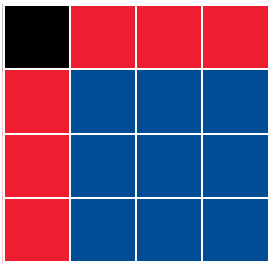
\includegraphics[width=.15\textwidth]
		{/home/deleonja/documents/docs_practicas/img-congreso/C0.png}
		\caption{}
	\end{minipage}\hfill
	\begin{minipage}[c]{0.5\textwidth}
		\centering
	  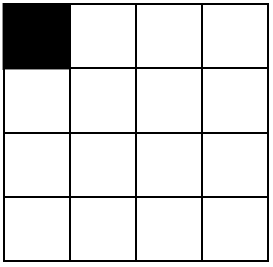
\includegraphics[width=.15\textwidth]
		{/home/deleonja/documents/docs_practicas/img-congreso/C16.png}
		\caption{}
	\end{minipage}
\end{figure}

\begin{figure}[H]
	\begin{minipage}[c]{0.5\textwidth}
		\centering
	  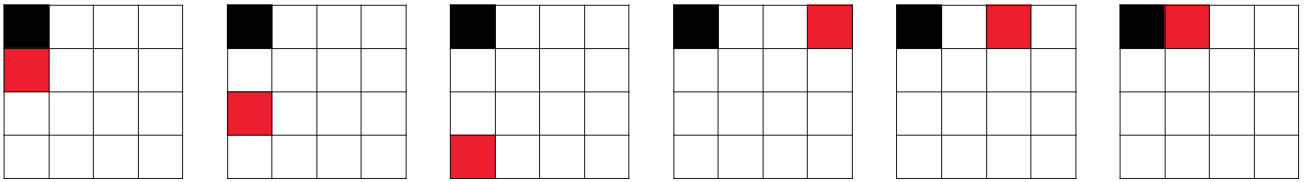
\includegraphics[width=.9\textwidth]
		{/home/deleonja/documents/docs_practicas/img-congreso/C12.png}
		\caption{C${}_1^2$}
	\end{minipage}\hfill
	\begin{minipage}[c]{0.5\textwidth}
		\centering
	  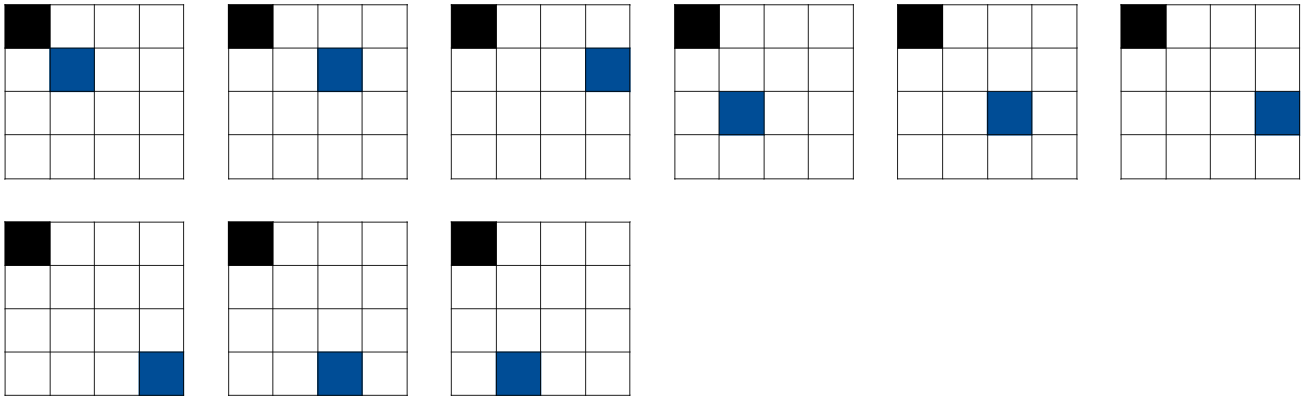
\includegraphics[width=.9\textwidth]
		{/home/deleonja/documents/docs_practicas/img-congreso/C22.png}
		\caption{C${}_2^2$}
	\end{minipage}
\end{figure}

\begin{figure}[H]
	\begin{minipage}[c]{0.5\textwidth}
		\centering
	  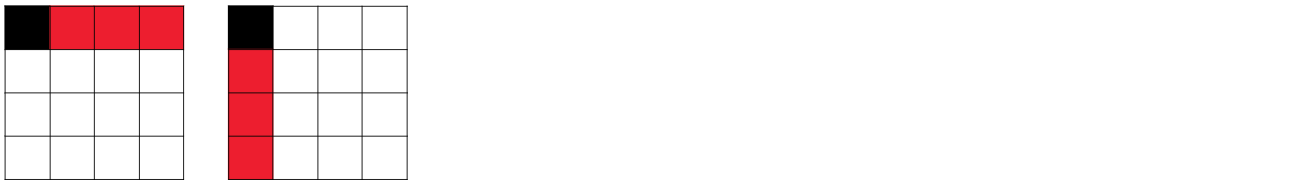
\includegraphics[width=.9\textwidth]
		{/home/deleonja/documents/docs_practicas/img-congreso/C14.png}
		\caption{C${}_1^4$}
	\end{minipage}\hfill
	\begin{minipage}[c]{0.5\textwidth}
		\centering
	  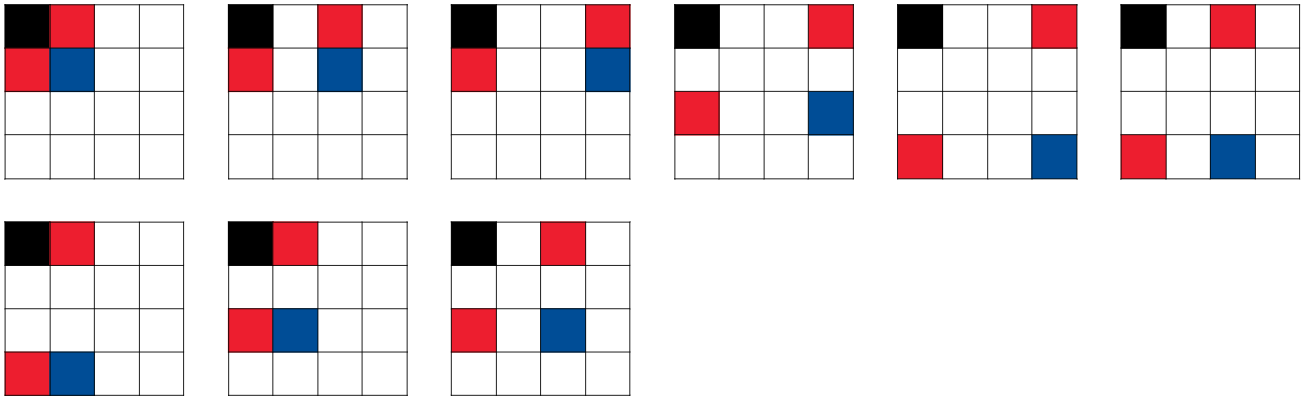
\includegraphics[width=.9\textwidth]
		{/home/deleonja/documents/docs_practicas/img-congreso/C24.png}
		\caption{C${}_2^4$}
	\end{minipage}\vfill
\begin{minipage}[c]{0.5\textwidth}
		\centering
	  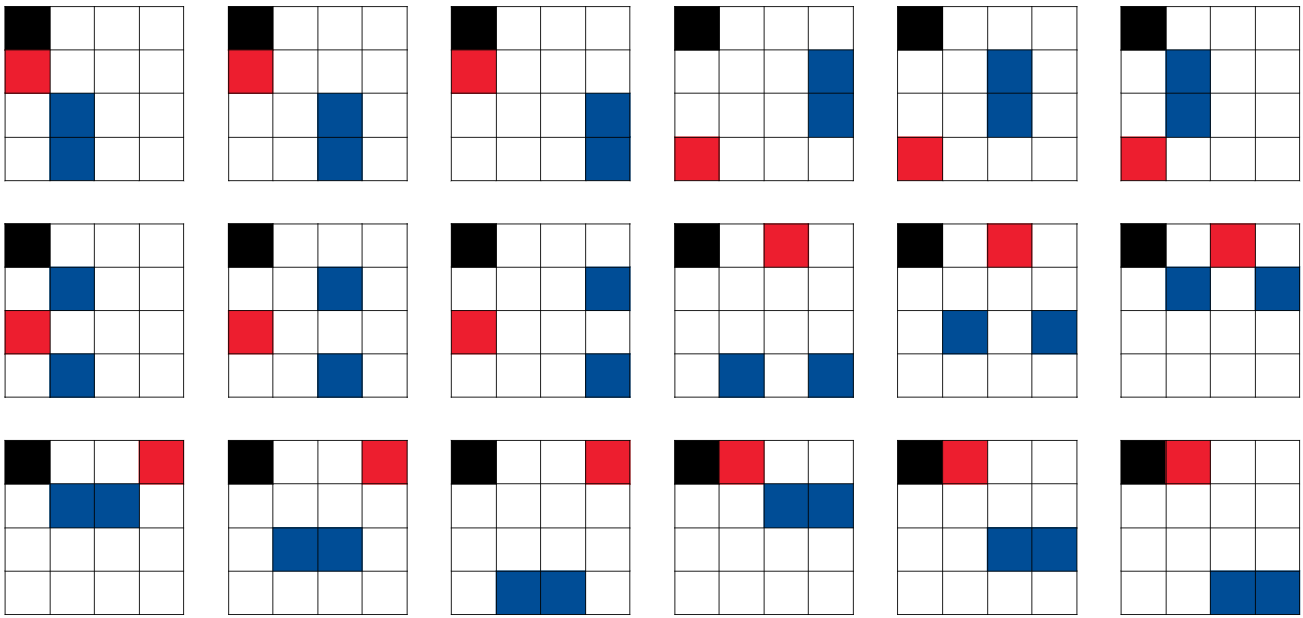
\includegraphics[width=.9\textwidth]
		{/home/deleonja/documents/docs_practicas/img-congreso/C34.png}
		\caption{C${}_3^4$}
	\end{minipage}\hfill
	\begin{minipage}[c]{0.5\textwidth}
		\centering
	  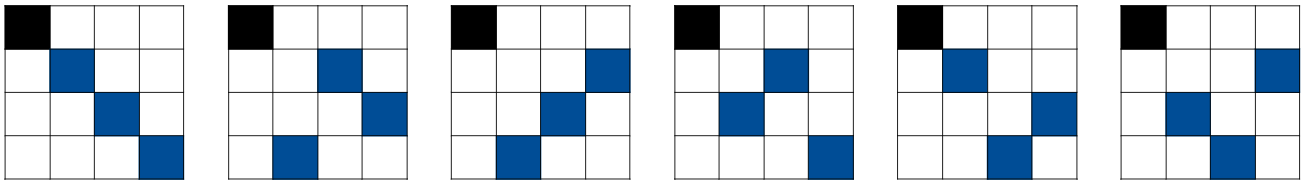
\includegraphics[width=.9\textwidth]
		{/home/deleonja/documents/docs_practicas/img-congreso/C44.png}
		\caption{C${}_4^4$}
	\end{minipage}
\end{figure}

\begin{figure}[H]
	\begin{minipage}[c]{0.5\textwidth}
		\centering
	  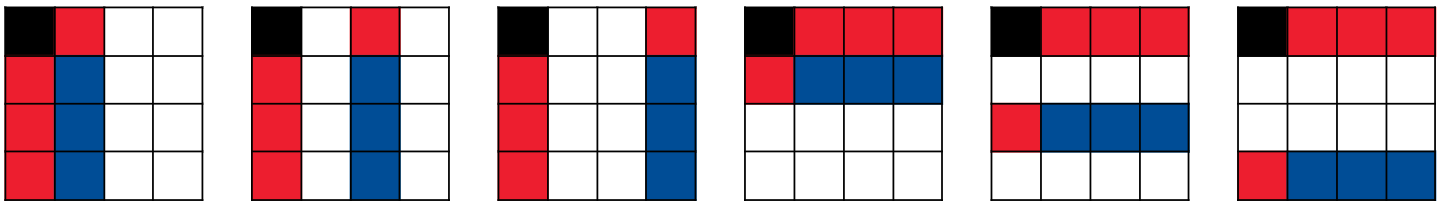
\includegraphics[width=.9\textwidth]
		{/home/deleonja/documents/docs_practicas/img-congreso/C18.png}
		\caption{C${}_1^8$}
	\end{minipage}\hfill
	\begin{minipage}[c]{0.5\textwidth}
		\centering
	  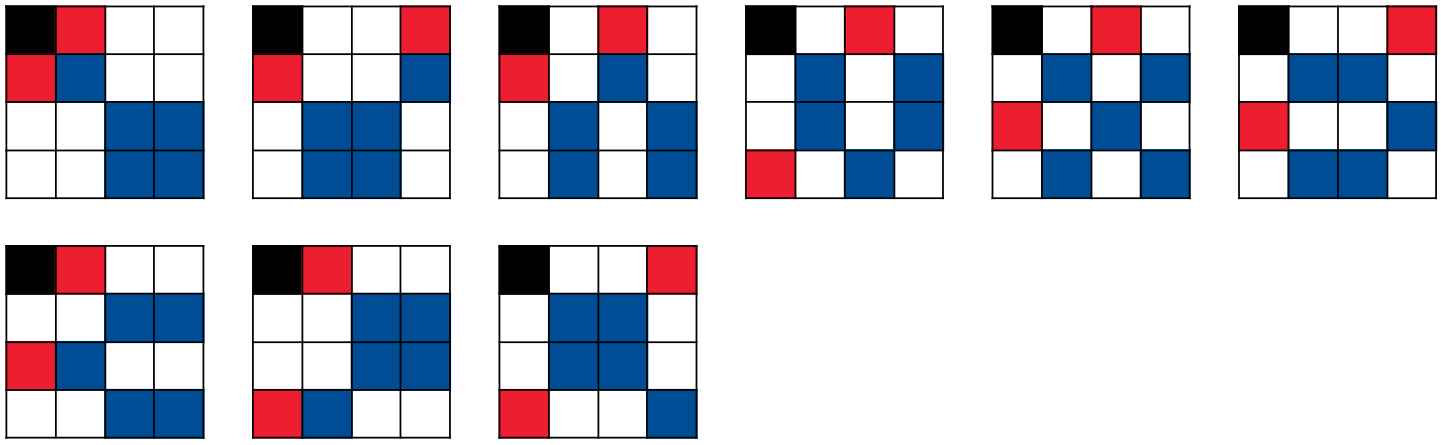
\includegraphics[width=.9\textwidth]
		{/home/deleonja/documents/docs_practicas/img-congreso/C28.png}
		\caption{C${}_2^8$}
	\end{minipage}
\end{figure}

\bibliographystyle{unsrt}
\bibliography{references}
\vfill

\end{document}
